\section{User interface design}
In this section are presented some mockups of the main features and related user interfaces the system is supposed to offer to the user and to the customer care through the proper web-based application. \\

The presented mockups have been designed based on both the \emph{PowerEnJoy: Requirements Analysis and Specification Document}\cite{RASD} and on the architectural design decisions and component interactions presented on this document. \\
In particular mockups show how the user interface is supposed to offer to the user the possibility to interact and make request to the system (obviously such user's interactions will result in a client-server communication of the user/customer care app view with the related server component based on the protocol chosen for that communication).  \\

The main goal of our mockups design process is to build an interface that clearly distinguish functionalities offered by the system taking into account the architectural decoupling offered by the taken design choices. \\

\clearpage

\subsection{User app}
The user app must have a charming and intuitive user interface in order to provide a easy-to-use experience to the user. The user app is supposed to be a web-based application, so the interface must be optimized for mobile devices even if the application is accessible and must be usable from every web browser on different size devices.

\subsubsection{Login page}
Simple initial page for the application to allow the user to authenticate to the system through username and password. A new user can access the registration process through the \emph{New User} button. \\
As specified in the requirements document, this page also allows a guest user or a \emph{banned} registered user to access to customer care contact information through the \emph{Contact us} button. \\
If a user is not recognized or is banned an error alert is shown when credential are submitted.

	\begin{figure}[h]
			\centering
			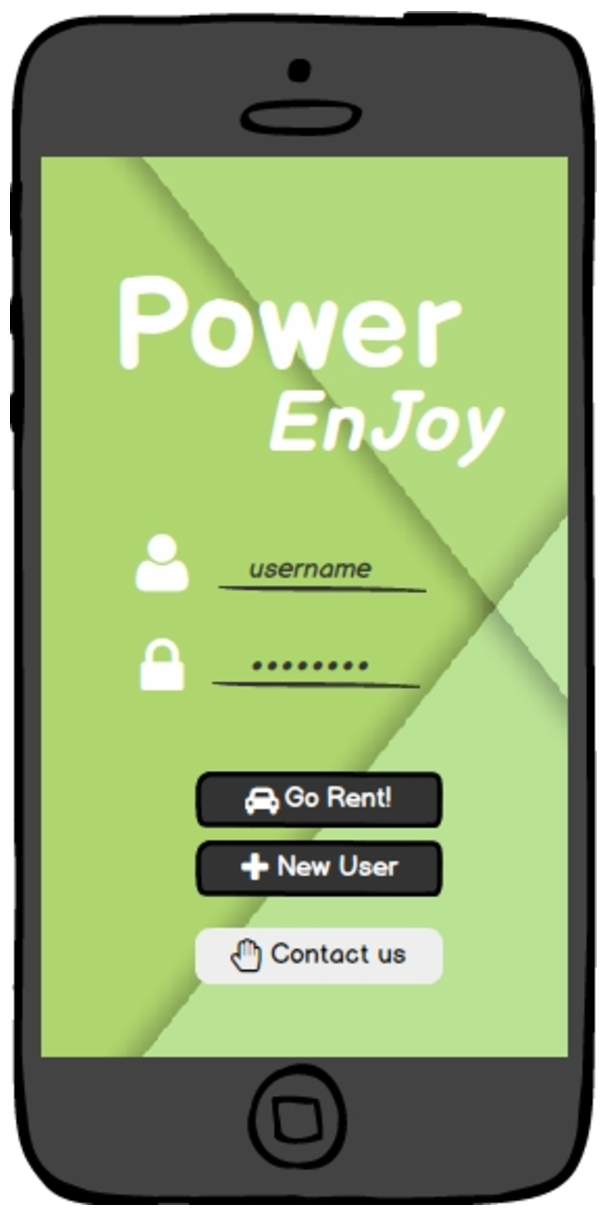
\includegraphics[width=0.4\linewidth]{mockups/loginPage}
			\caption{
				\label{fig:loginPage} 
				\emph{Login page} mockup
			}
		\end{figure}
		
\clearpage

\subsubsection{Home page}
The home page shows to a logged user all the possible functionalities provided from the app:
\begin{itemize}
	\item See available cars and reserve one of them (eventually with the \emph{money saving option})
	\item Unlock a car (disabled button in the mockups, it would be active only if there is an active reservation for the registered user logged in)
	\item See user's information and edit them
	\item See user's rent history
	\item See user's payment history
	\item Show customer care contact information
\end{itemize}

This page shows also the user's name to ensure to the user he has been correctly recognized by the system and to make the interface more customized. \\

The icon in the right corner, from this page, brings the user to the functionality of see available cars; on all other pages (without the orange position icon) it brings the user to this page: the home page.

	\begin{figure}[h]
			\centering
			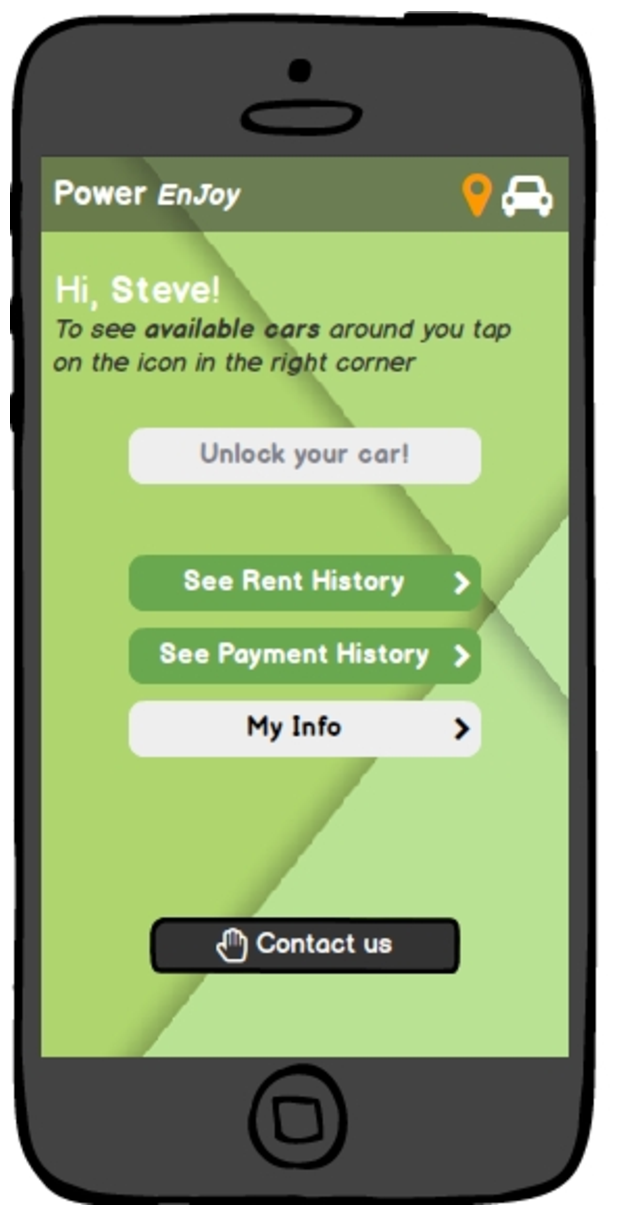
\includegraphics[width=0.4\linewidth]{mockups/homePage}
			\caption{
				\label{fig:homePage} 
				\emph{Home page} mockup 
			}
		\end{figure}
		
\subsubsection{See available cars}
Accessing to the see available cars functionality, as described in the requirements document, the user app asks to the user if he wants to search car nearby his actual position (using GPS position of user's device) or he wants to insert a different position from which starting the research. \\

The \emph{Use GPS} allows the user to choose the first option skipping other interactions on this page. \\

If the user chooses the second option, he is supposed to insert an address location (e.g. 34 Maria Victoria Lane, London) before pushing the \emph{Search} button; the system will resolve that address as a GPS location displaying an error message if it could not done it. \\

The \emph{Cancel} button allows the user to return to the home page. \\

The system searches for available cars (nearby the position given by the user or retrieved by the GPS) and displays a map with available cars on their actual position, charging station positions (green spot) and safe areas (black areas). Blue circled cars are actually plugged on a charging station, all others car are green circled.\\

The map is interactive and the user can move around the actual position. \\

	\begin{figure}[h]
			\centering
			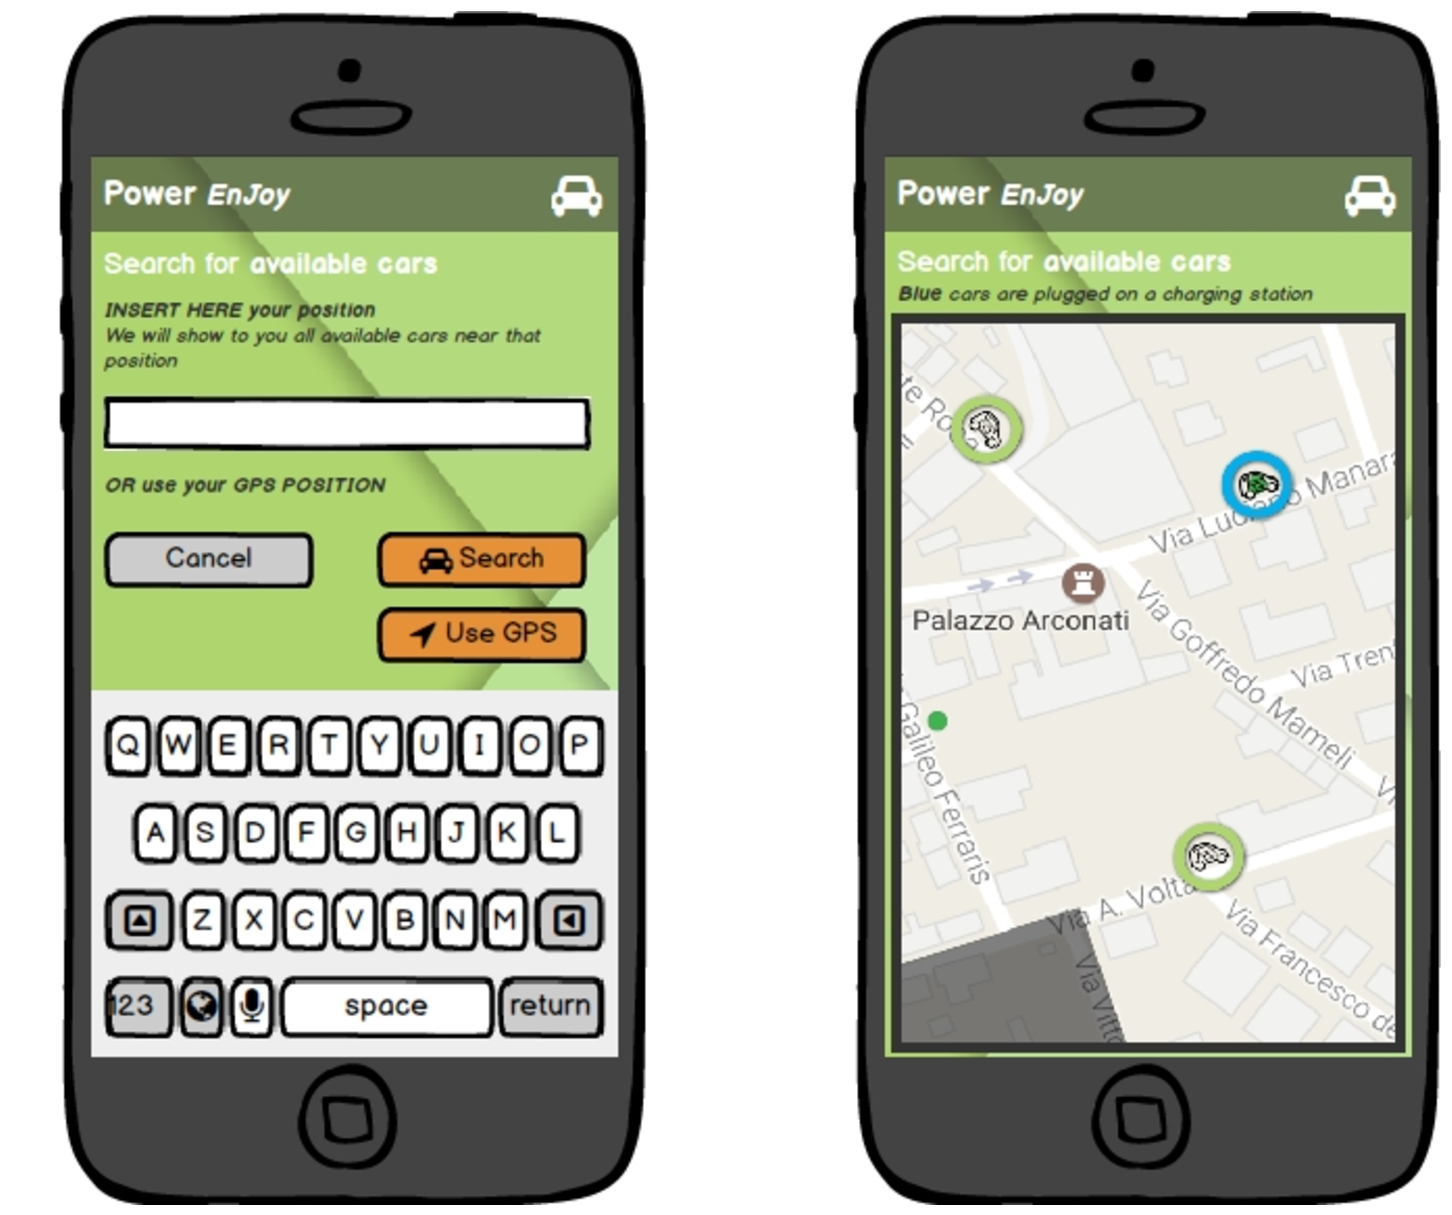
\includegraphics[width=0.9\linewidth]{mockups/findCar}
			\caption{
				\label{fig:searchCar} 
				\emph{See available cars} mockup
			}
		\end{figure}

\subsubsection{Reserve a car}

From the page showing available cars on the map, a user tapping on a car could access information about it, in particular:
\begin{itemize}
	\item Model of the car
	\item License number of the car
	\item The battery percentage level of the car
\end{itemize}

When the user taps on a car the circle around it becomes orange, to give a feedback on the tap to the user, and a box appears on the screen. Through it the user can access the aforementioned info about the car and reserve the selected car. \\

Before clicking the \emph{Reserve it!} button the user has the possibility to choice if he wants or not to enable the \emph{money saving option} through an on/off toggle.\\

If a user has already an active reservation or the selected car has been reserved while the user navigates on the map an error message is displayed.\\

\begin{figure}[h]
			\centering
			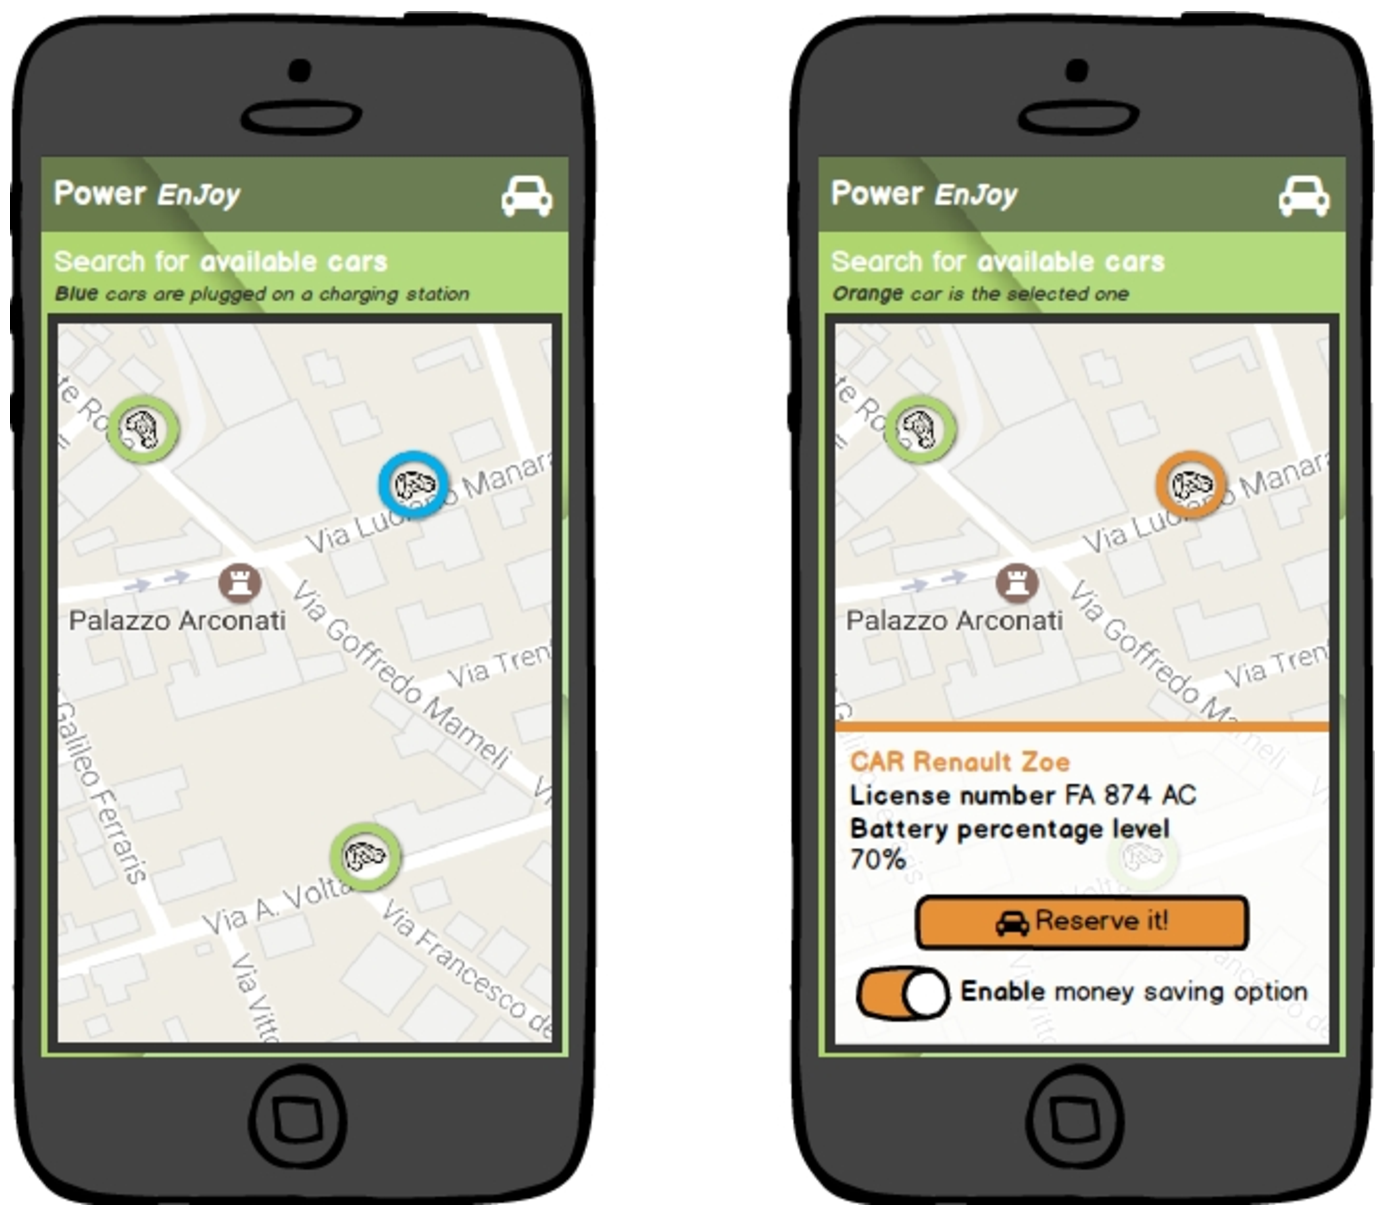
\includegraphics[width=0.9\linewidth]{mockups/reserveCar}
			\caption{
				\label{fig:reserveCar} 
				\emph{Reserve a car} mockup
			}
		\end{figure}
		
\subsubsection{Money saving option}

If an user enables the \emph{money saving option} while reserving a car, the user app shows him a dedicated page to accomplish the reservation with the option. On this page the user must insert the planned destination of his rent in order to give to the system the possibility to calculate the charging station the user must leave the car plugged in to get the discount.\\

A brief description of the \emph{money saving option} is offered to the user to clarify why the user app is asking him his planned destination. \\

The user is supposed to insert an address location (e.g. 34 Maria Victoria Lane, London) before pushing the \emph{Confirm} button; the system will resolve that address as a GPS location displaying an error message if it could not done it. \\

If the address inserted by the user is correctly processed the system notifies the user with the charging station (number and address) 
the user must leave the car plugged in to get the discount. \\

The \emph{Cancel} button allows the user to go back on the map, for example to make the reservation without enabling the \emph{money saving option}.

\paragraph{Note} Note that if the user chooses to enable the \emph{money saving option} the car reservation request is sent to the server only when the user inserts also the destination.

\begin{figure}[h]
			\centering
			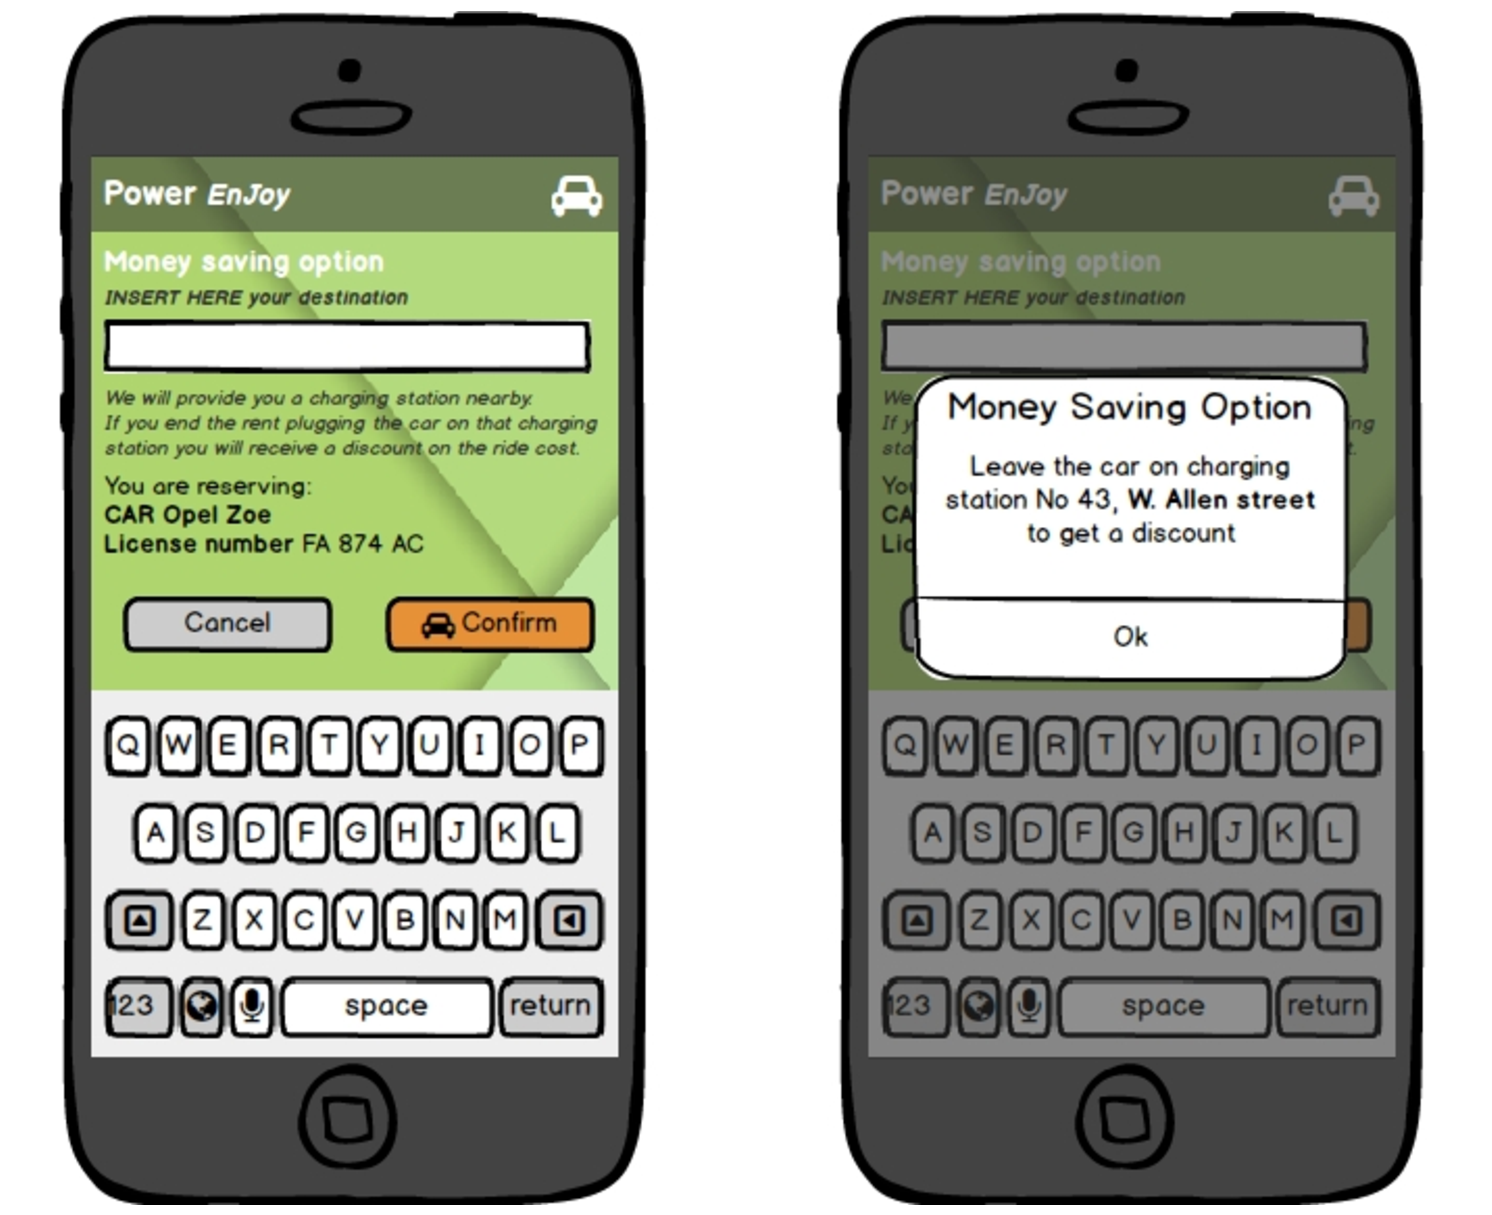
\includegraphics[width=0.9\linewidth]{mockups/moneySavingOption}
			\caption{
				\label{fig:msOption} 
				\emph{Money saving option} mockup
			}
		\end{figure}

\subsubsection{Unlock a car}

From the home page, if the user has an active reservation he can access to the \emph{Unlock car} functionality through the dedicated button. \\

On this page the user can see data about his reservation:
\begin{itemize}
	\item model and license number of the car he has reserved
	\item time until the reservation expires
	\item (\emph{Optional}) charging station related to money saving
	 option
	\item  current car position (clicking on \emph{see it on the map} link the user app looks for an installed program on the user device to open the GPS coordinates, if it can not find any program it only shows the GPS coordinates)
\end{itemize}

The user could ask the system to unlock the car through the \emph{Unlock your car} button. If the user GPS position is not 5m away from the car an error message is displayed to ask the user to reach the car before trying to unlock the car. \\

If the system manages to process the request to unlock the car a message is displayed to notify the user the car has been unlocked and he could start the rent turning on the engine.\\

\begin{figure}[h]
			\centering
			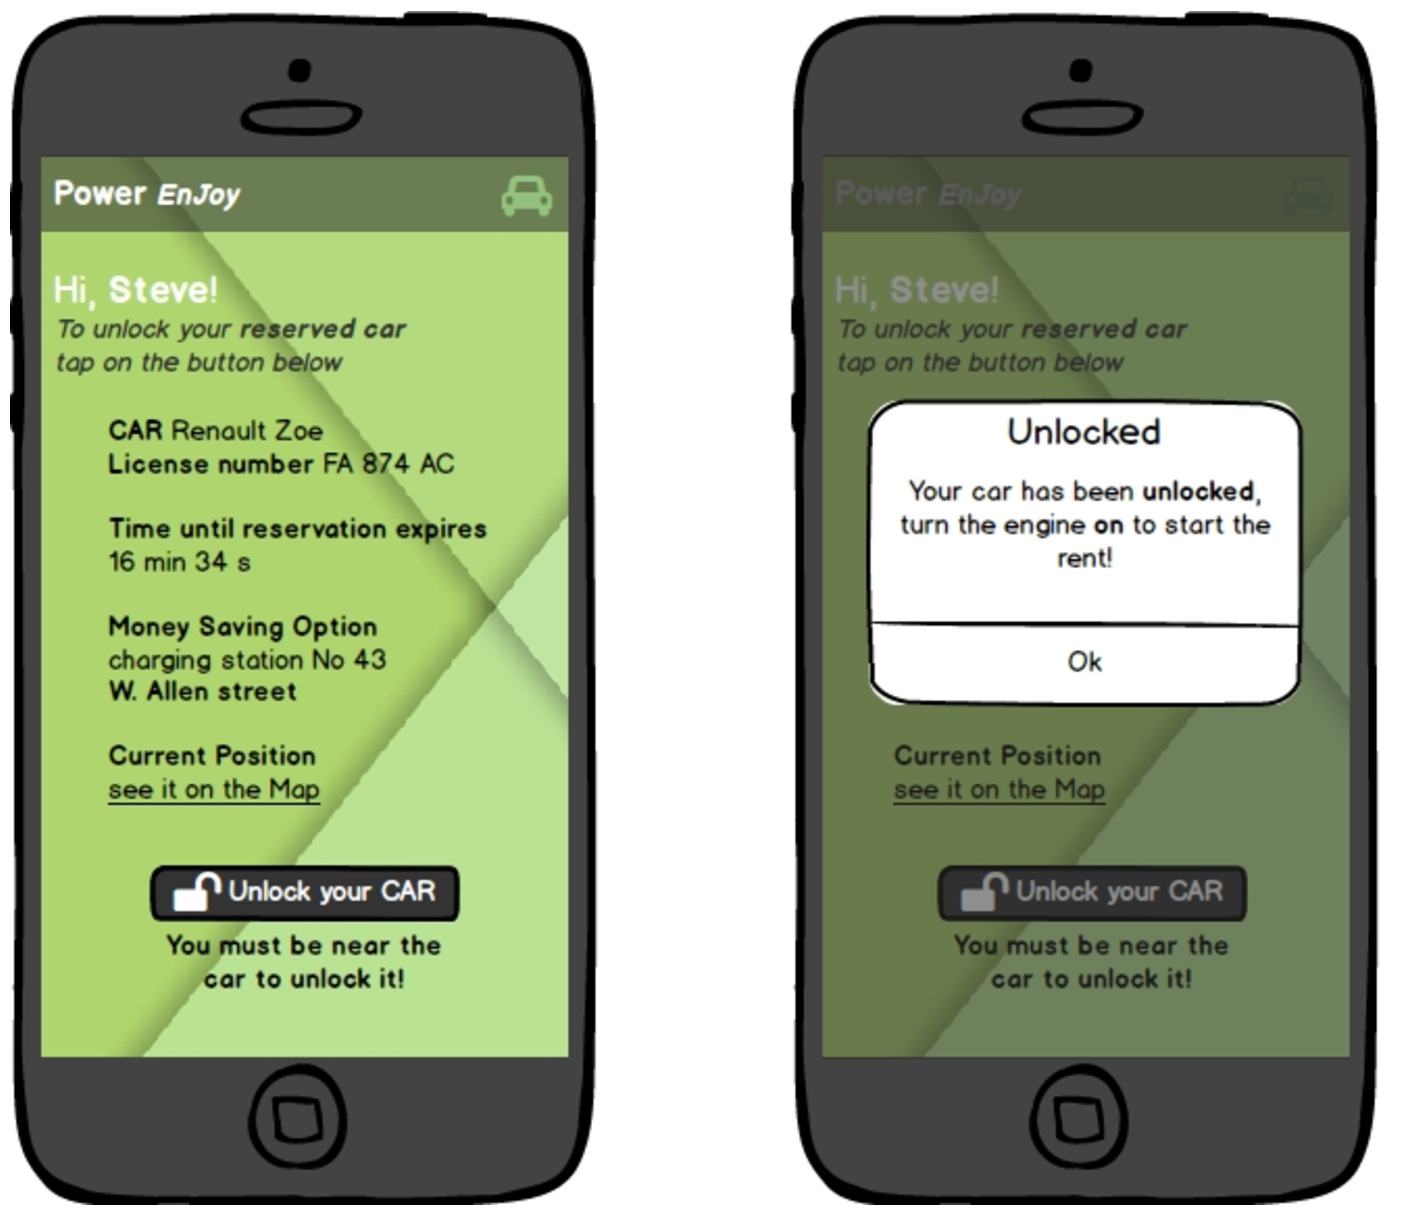
\includegraphics[width=0.9\linewidth]{mockups/unlockCar}
			\caption{
				\label{fig:unlockCar} 
				\emph{Unlock a car} mockup
			}
		\end{figure}

\subsubsection{Payment history}

From the home page, the user can access his own payment history through the \emph{See Payment History} button. \\

On this page the user app shows to the user all made payments in chronological order, from the more recent to the latest ones as shown in \autoref{fig:paymentHistory}. \\

Payment not related to a rent, for example fee related to an expired reservation, are shown with a different color to clearly distinguish it. \\

Through this page a user can only see if a payment is related or not to a rent and date and hour of each payment. The user could access all payments details clicking on one of the rows shown, or can rapidly access to customer care contact information if for example it finds out some payment he is not aware of. \\


\begin{figure}[h]
			\centering
			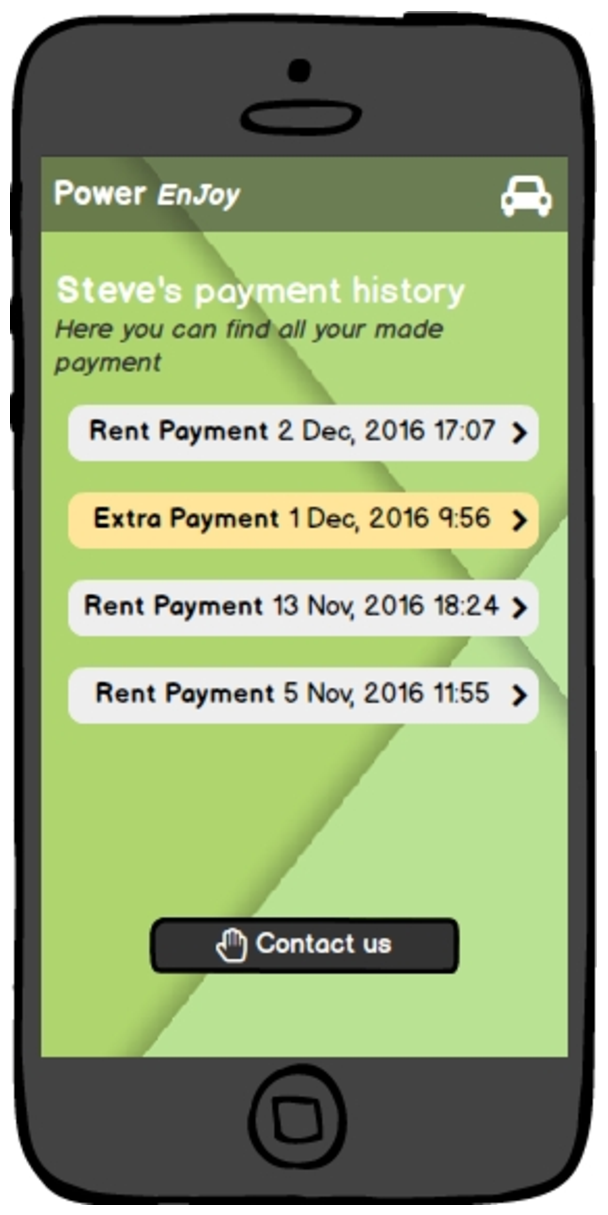
\includegraphics[width=0.4\linewidth]{mockups/paymentHistory}
			\caption{
				\label{fig:paymentHistory} 
				\emph{Payment history} mockup
			}
		\end{figure}
\clearpage

In \autoref{fig:payments} are shown two examples of payments history's single record. The one on the right shows a payment related to a rent, instead the one on the left shows a payment related to a reservation expired fee. \\

For each payment record the user can see information about:
\begin{itemize}
	\item payment ID
	\item time of the payment
	\item base cost (in case of rent it's calculated as \emph{rent time} x \emph{time based rate})
	\item discount amount applied on the rent 
	\item fee amount applied on the rent
	\item total paid amount
	\item payment used method (for security reason only the last four numbers are shown)
	\item (\emph{optional}) rent associated with the payment
\end{itemize}

If the payment is associated with a rent, the user can access the rent record through the link in the \emph{rent} section.
\\
 
\begin{figure}[h]
			\centering
			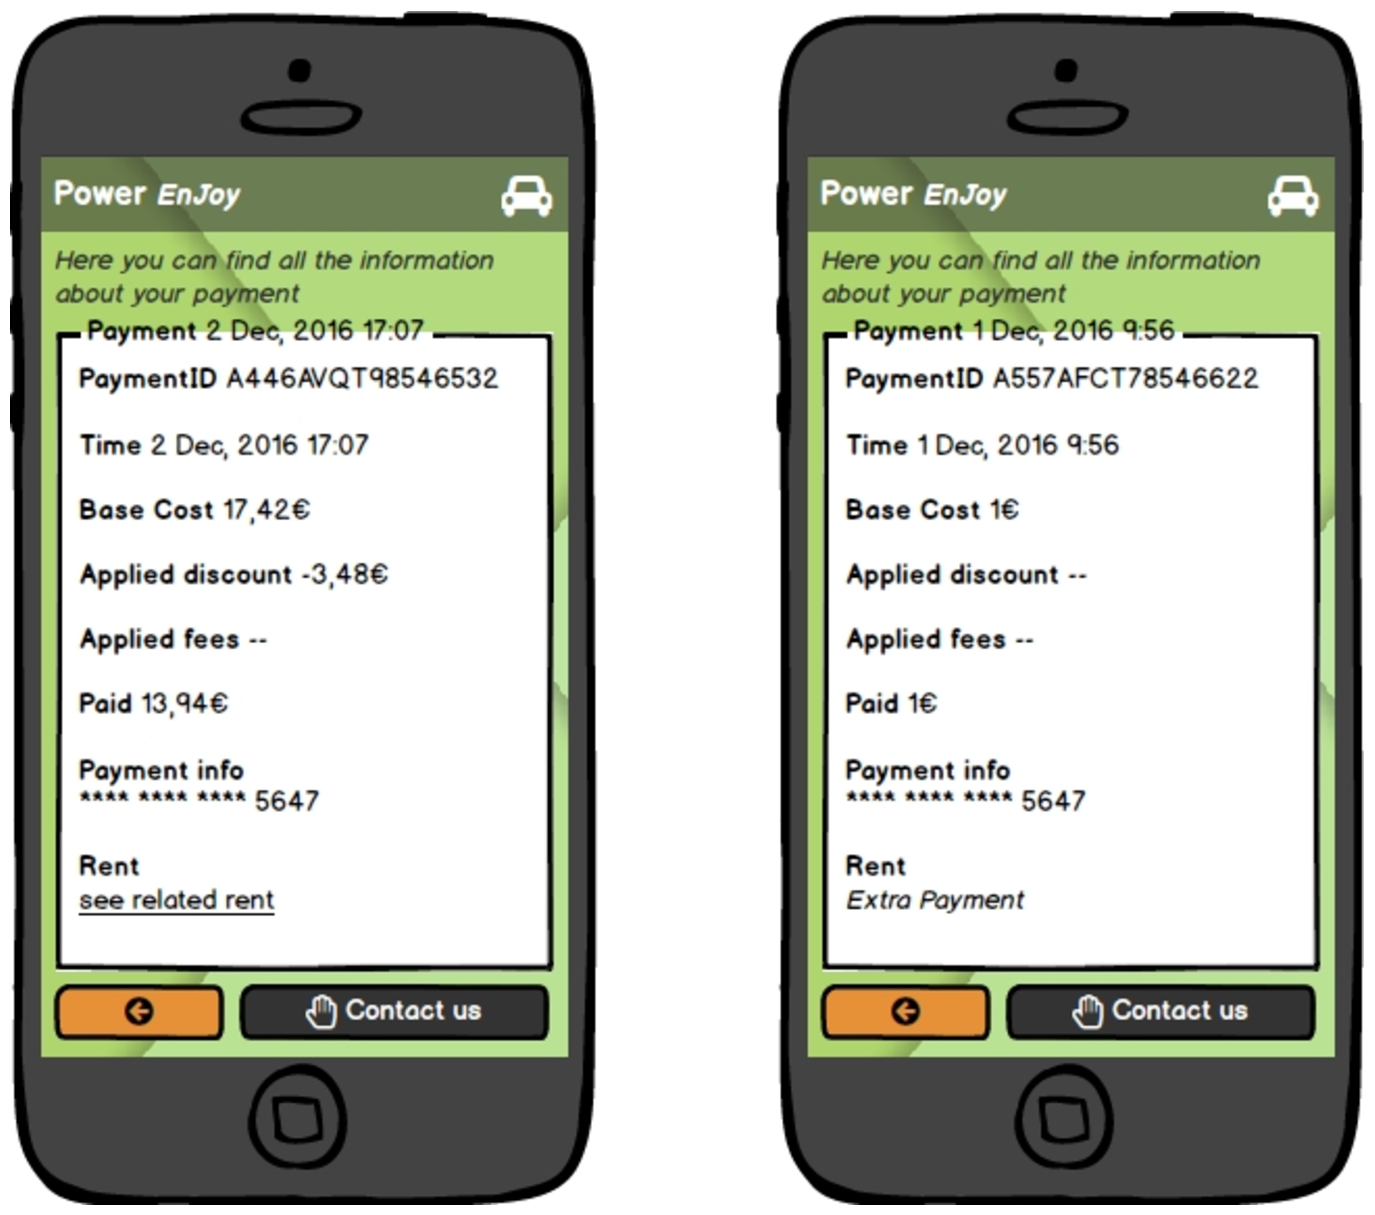
\includegraphics[width=0.9\linewidth]{mockups/payments}
			\caption{
				\label{fig:payments} 
				\emph{Single payment records} mockup
			}
		\end{figure}

\clearpage

\subsubsection{Rent history}

From the home page, the user can access his own rent history through the \emph{See Rent History} button. \\

On this page the user app shows to the user all made rents in chronological order, from the more recent to the latest ones as shown in \autoref{fig:rentHistory}. Through this page a user can only see date and hour of each rent. The user could access all rents details clicking on one of the rows shown. \\

For each rent record the user can see information about:
\begin{itemize}
	\item rent ID
	\item start/end time and location of the rent
	\item all discount applicable to the rent
	\item all fee applicable to the rent
	\item payment related to the rent
\end{itemize}

The user can access the payment record related to the rent through the link in the \emph{payment} section.
\\

\begin{figure}[h]
			\centering
			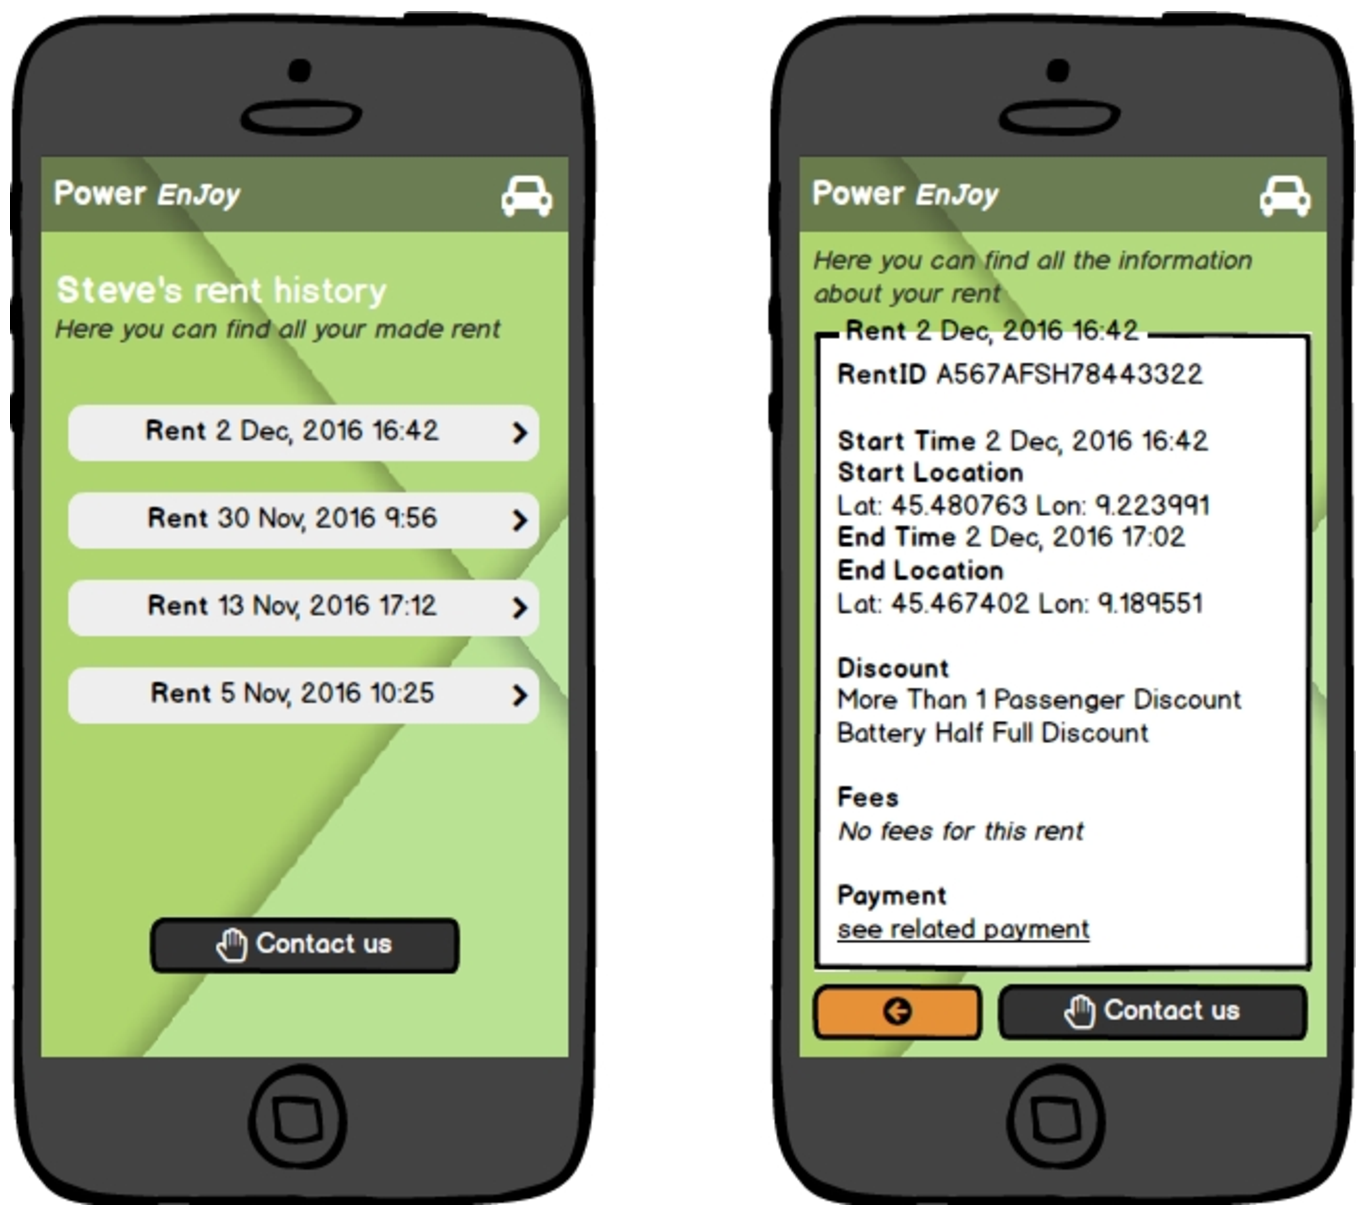
\includegraphics[width=0.9\linewidth]{mockups/rentHistory}
			\caption{
				\label{fig:rentHistory} 
				\emph{Rent history} mockup
			}
		\end{figure}

\clearpage

\subsection{Customer care app}
The customer care app has a simple interface in order to provide features to customer care operator in a clear and simple way. This interface must be optimized for a desktop monitor size.

\subsubsection{Home page}
All main features are accessible directly from the home page to provide a rapid and intuitive access to them. \\
From the home page the operator can:
\begin{itemize}
	\item Access information about a user through the user's username or email address (see \hyperref[sec:userInfoCc]{user's information section}) 
	\item Mark/Unmark user as banned through its username (if the username inserted is found by the system, in order to fulfil this task a new page is shown otherwise a new error message is displayed. The new page shows to the operator the current state of the user and if the operator wants to mark the user as \emph{banned} asks the operator a brief description of the reasons)
	\item Retrieve basic data for each user (username, name, surname, email)
	\item Tag a car as \emph{Not Available} (if the car license number inserted is found by the system, in order to fulfil this task a new page is shown otherwise a new error message is displayed. The new page  asks the operator a brief description of the reasons why he wants to mark the car as {Not Available})
\end{itemize}
 
 \begin{figure}[h]
			\centering
			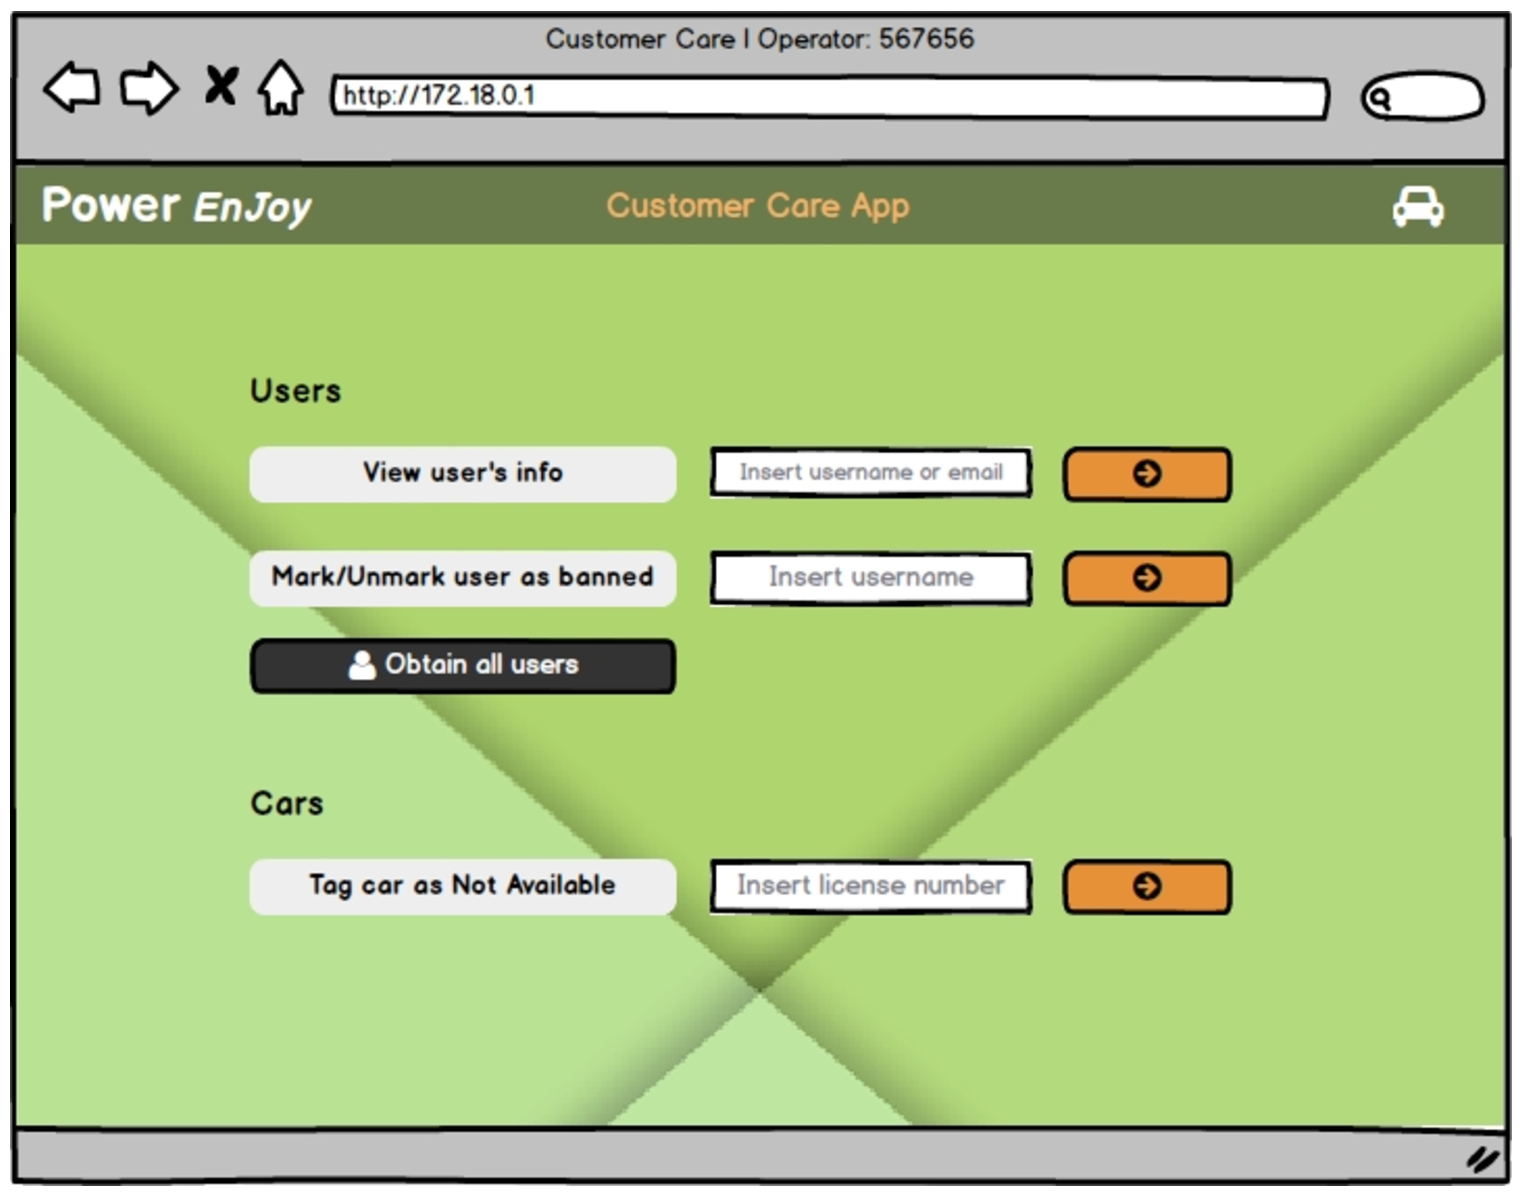
\includegraphics[width=0.895\linewidth]{mockups/customerCare1}
			\caption{
				\label{fig:cc1} 
				\emph{Customer care home page} mockup
			}
		\end{figure}

\clearpage 
		
\subsubsection{User's information} \label{sec:userInfoCc}

From the home page the operator could access information about a specific user. In this page the customer care app shows to the operator all user's information unless the sensitive ones (as password and credit car number). \\

From this page the operator could also access user's rent and payment history through specific buttons.

\begin{figure}[h]
			\centering
			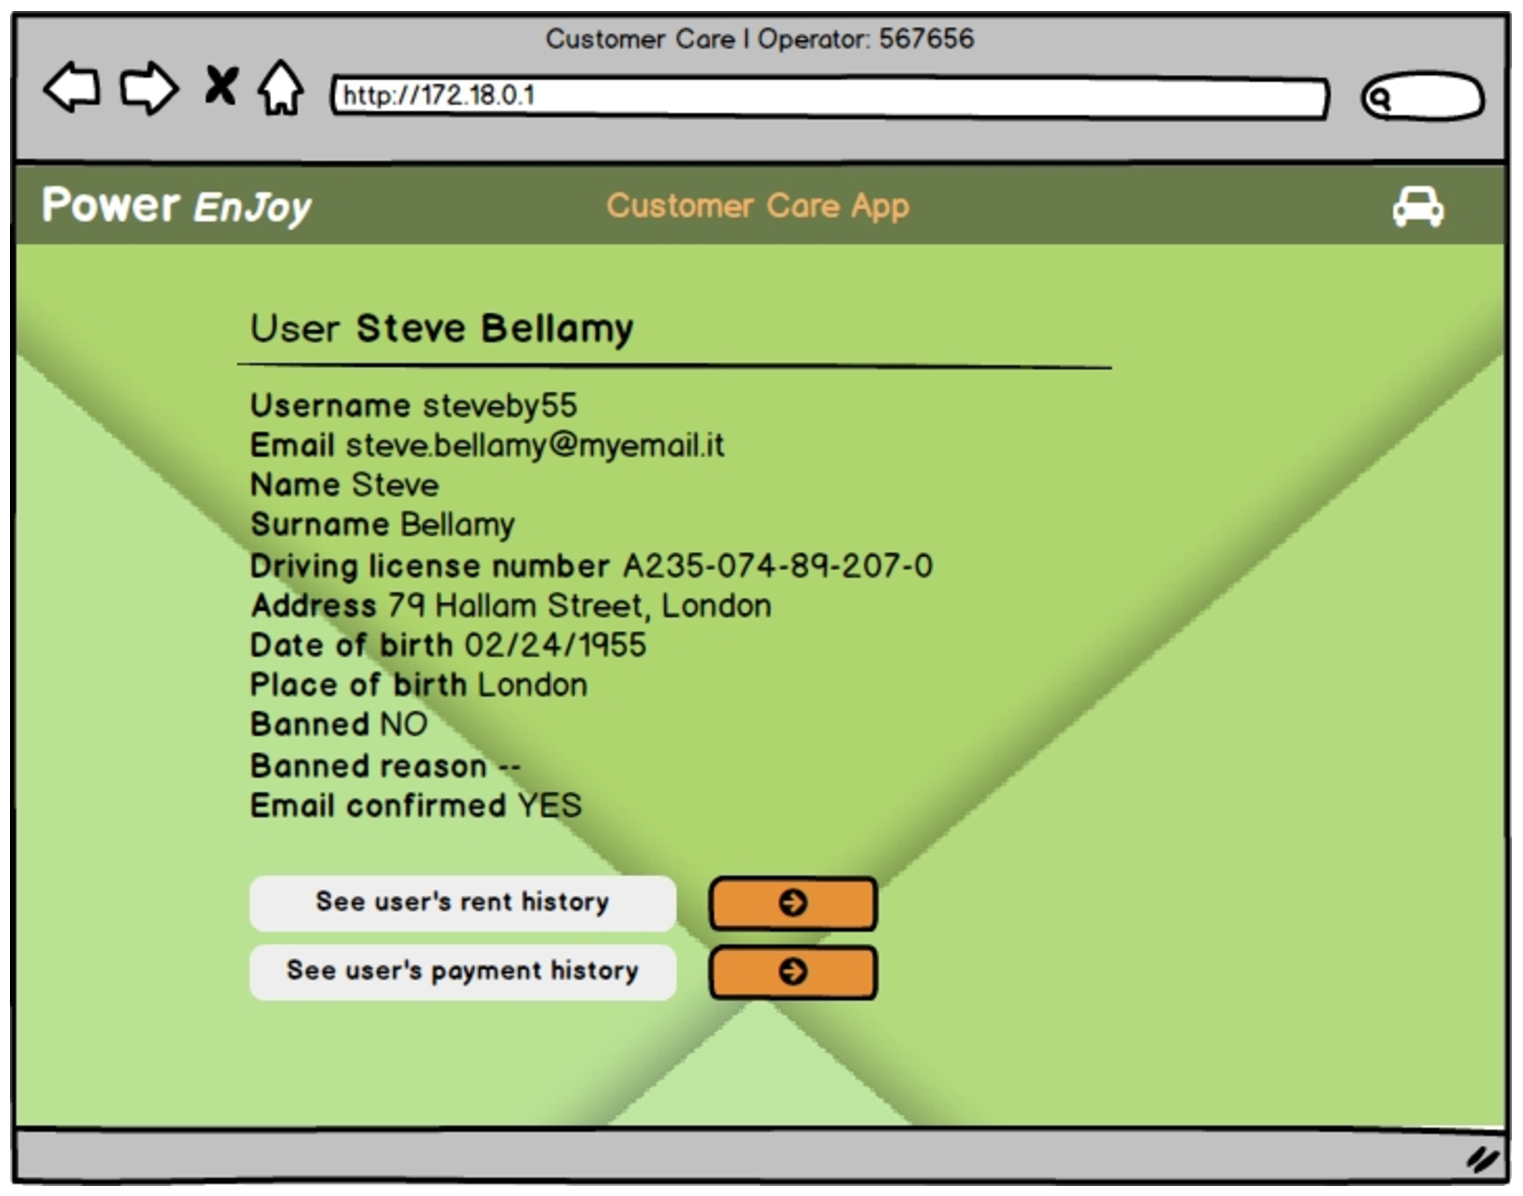
\includegraphics[width=0.895\linewidth]{mockups/customerCare2}
			\caption{
				\label{fig:cc2} 
				\emph{Customer care user's information page} mockup
			}
		\end{figure}